\subsection{Introduction to the Choicely voting platform}
    % what does the company do? 
    Choicely \footnote{\url{http://choicely.com/}} is a voting platform developed by a Finnish startup, Lovented Ltd, since 2014. The software provides the possibility for users to engage in interesting contests by voting on their favorite contender. The platform has already hosted numerous contests in various fields, such as beauty pageants, public polls, design contests, sport events among many others. The customer base of the firm consist of mainly Finnish broadcasters, publishers and advertisers. However, the last year has brought numerous users and customers from all around the world.
    
    % what are the contests like, what kind of configuration settings are available?
    % The contests in the platform are created by users or brands. 
    Contests can be of multiple types: ... % TODO ask Kaius 
    
    % voting options
    Various voting options are available for contests. The author of the contest has the choice of setting a limit on how many votes users can spend on individual participants or the whole contest in overall. For instance, if the maximum votes in the contest is set to 1, users can give exactly one vote on exactly one participant. Configuration settings allow infinite votes as well. Removing votes is possible, if the author has decided to enable this possibility. Votes cannot be modified after the contest has ended.
    
    % free-silver-gold votes
    On top of the regular free votes, contest authors may allow users to earn more votes (called "silver votes") by sharing the contest on social media or by watching advertisements. Furthermore, authors can allow users to purchase more votes (called "star votes" or "gold votes") with exactly the same restriction settings as explained above. Note, however that the configuration for the three vote types are distinct for every contest. This means that the limitation on free/silver/star votes may differ for individual participants as well as the whole contest. 

    % how can one reach a contest in the platform?
    Contests can be accessed through multiple interfaces (Figure \ref{choicely_platforms}). Naturally, the company's webpage provides a convenient way to create, browse and participate in contests. Choicely also has free mobile applications available on Android and iOS devices, that can be installed through the Google Play \footnote{\url{https://play.google.com/store/apps/details?id=com.choicely.android}} and the iOS App Store \footnote{\url{https://itunes.apple.com/fi/app/choicely/id1158798364}} on the devices. Finally, the company offers a web widget, which can be embedded as a framework in any webpage easily. The last option is often used by many of Choicely's customers, because it provides a convenient way to embed rich content in their own web pages.
    
    % what do users have to do to participate? 
    Majority of the contests require users to have a user profile in the Choicely platform. Optionally, profiles can be created through a regular sign-up process, where users register and pick a password for their authentication. When users choose this kind of registration, their e-mail addresses are confirmed through a verification link sent to their inbox, so that their identity is confirmed.      

    \begin{itemize}
        \item Full name
        \item Profile picture
        \item Cover image
        \item Gender
        \item Location (Country, state and city)
        \item Age group
        \item Introduction/Bio
    \end{itemize}

    % what is the connection between contests and users? How do the participate?
    Users may vote and participate in their own contests if they like. Users may participate in arbitrary number of contests from three platforms: the two most popular mobile platforms (iOS and Android) and the web interface (Figure \ref{choicely_platforms}). 
    
    \begin{figure}[h] 
        \begin{center}
            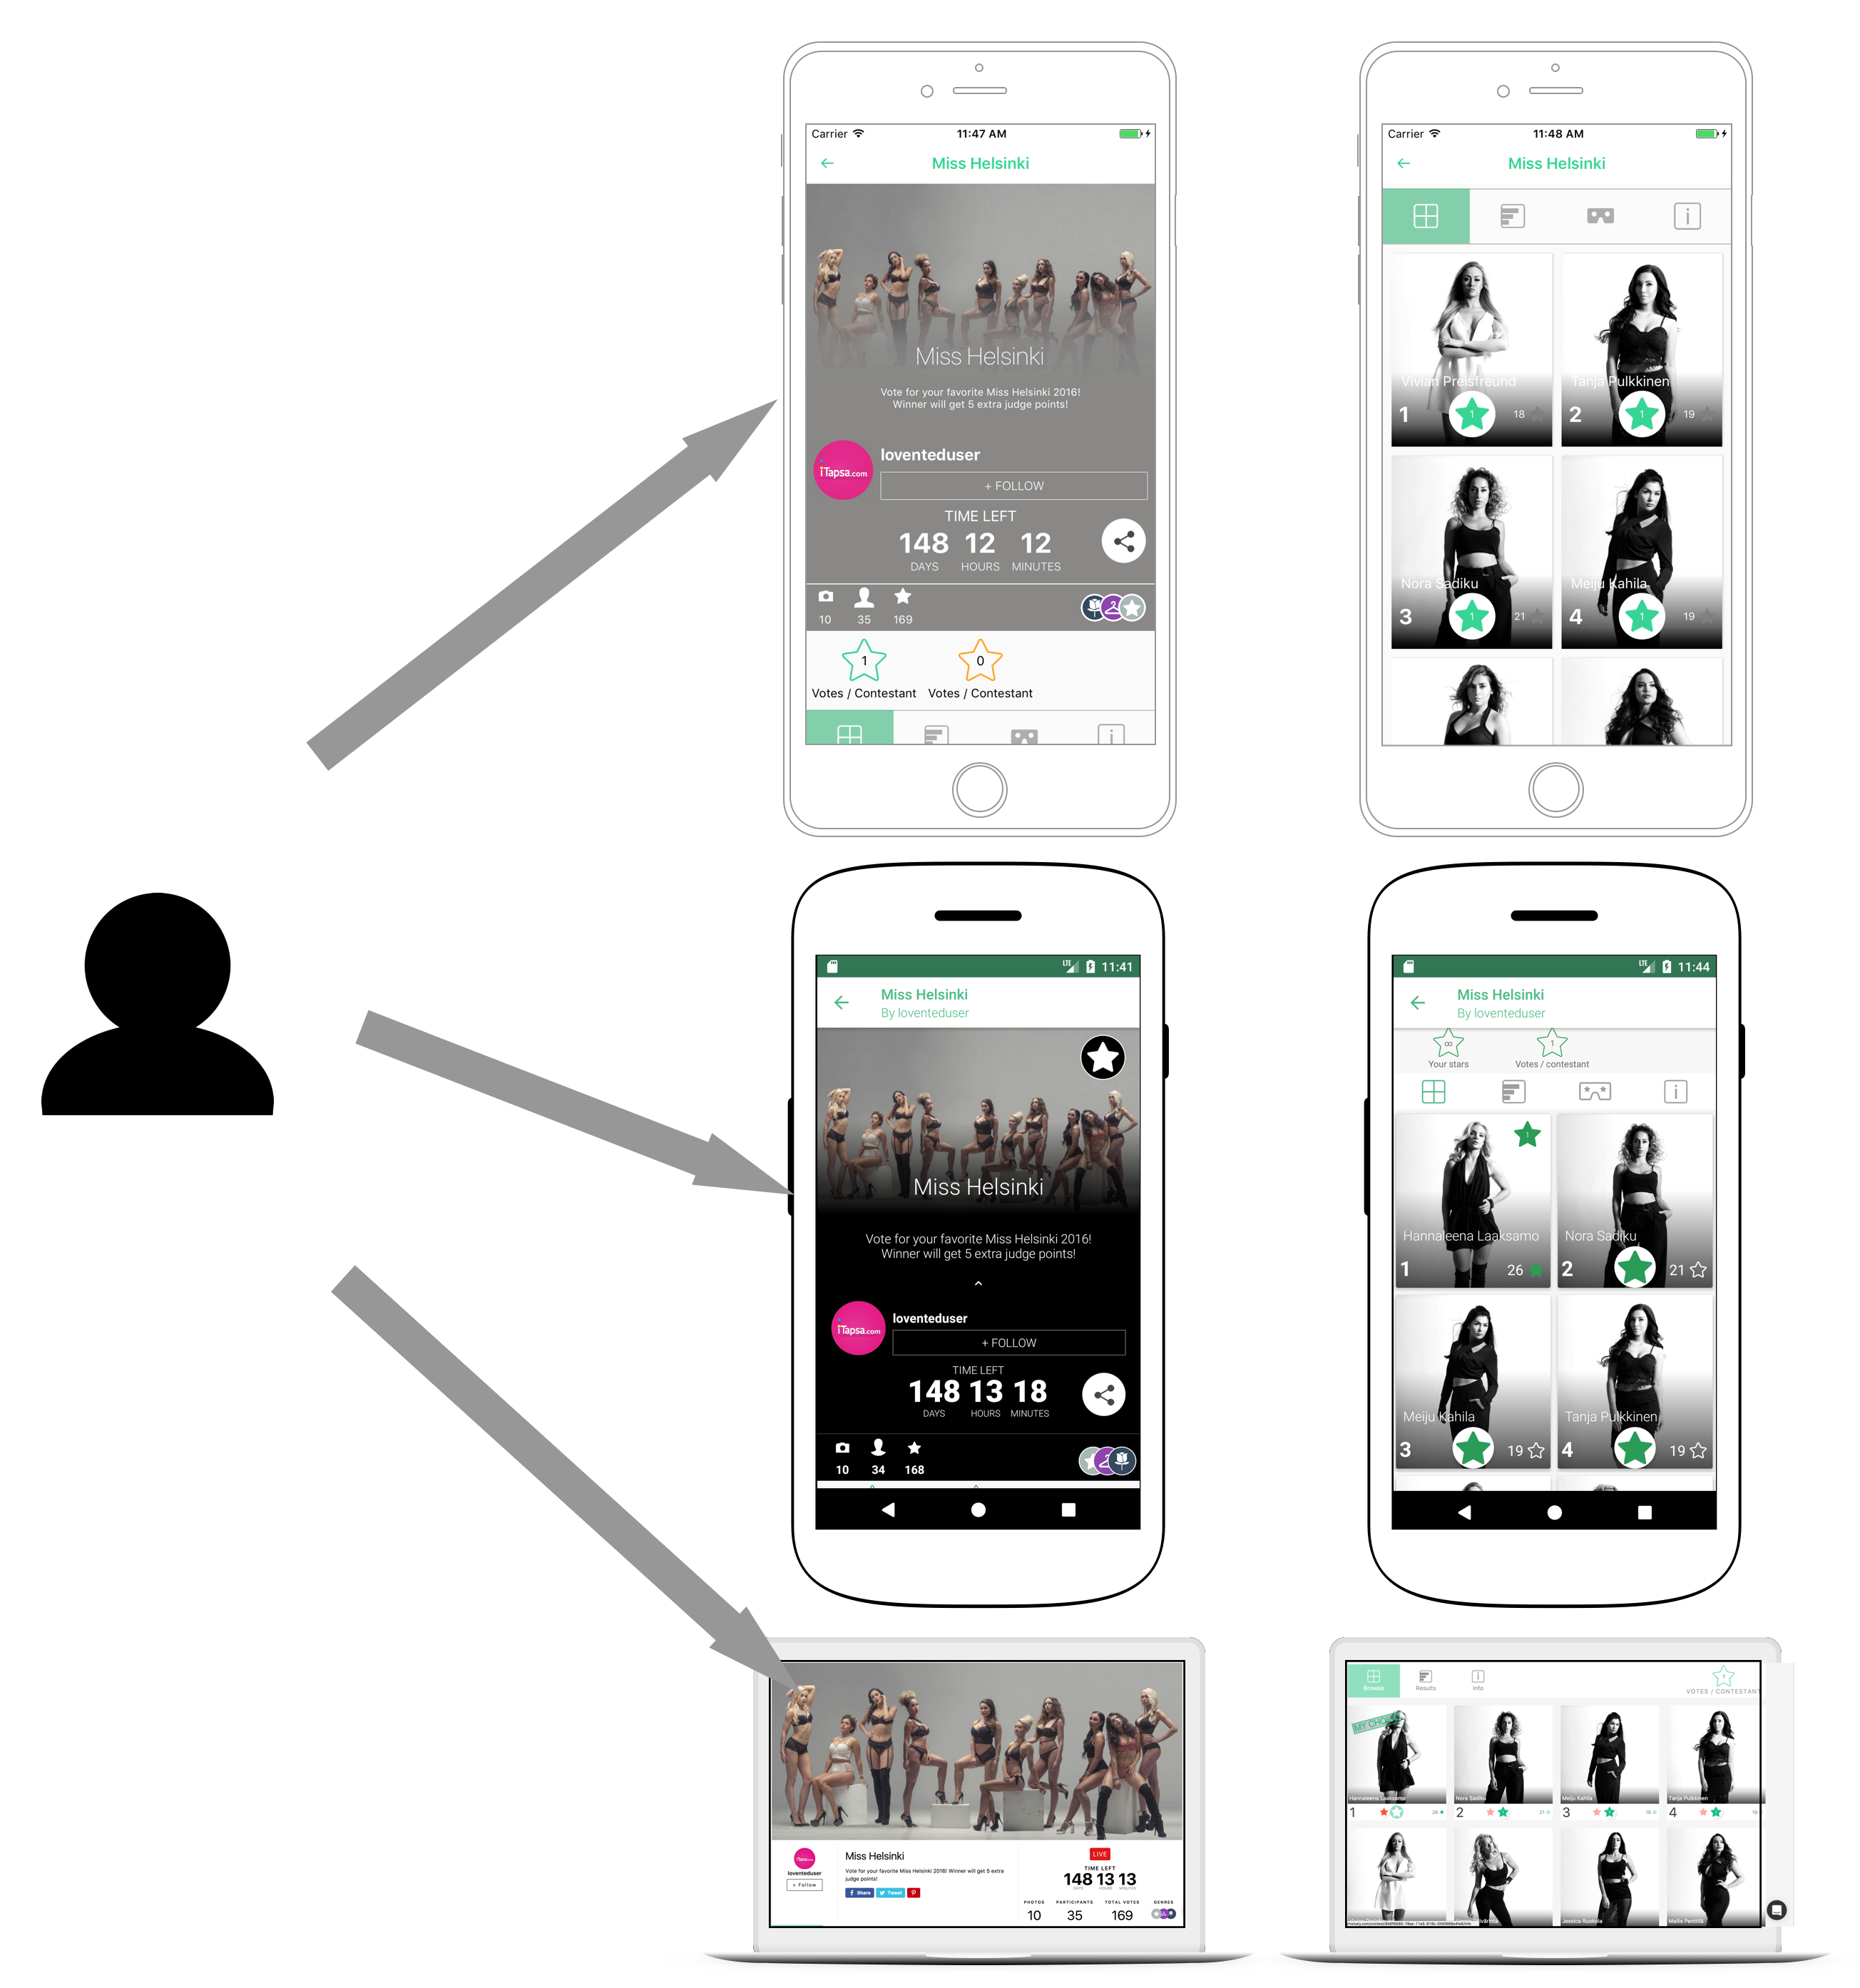
\includegraphics[width=0.6\textwidth]{images/choicely_platforms.png}
            \caption{Users can vote in contests through three interfaces: iOS devices, Android devices and web.}
            \label{choicely_platforms}
        \end{center}
    \end{figure}

    % what kind of data is generated?
    The available data is two-folded: each user has a user profile, which contains basic demographic information about the user (gender and location), while contests have a number of participants with arbitrary number of votes that the users have spent on them. The vote changes for the contests are stored as transactions. This means that the database contains not the final results of the voting, but rather the changes what users made while using the software. This way it is possible to analyze the votes over time and to look at changes individually. For instance, it is possible to tell if a user has removed his/her votes from participant A and moved them to participant B. Furthermore, this way of data representation to restore or simulate any previous state of the contest, in case it would be needed.

    % how does the data look like and how can it be retrieved?
    The data is structured in nature and is stored in a... The data can be accessed via...

    %  why is it important to analyze this kind of data and what can we learn from it? 
    There is a need to analyze this data, because...
    
\subsection{Research setting}
    % why is the data analysis relevant from scientific research point of view?
    Performing scientific research on such data is interesting for multiple reasons. To begin with, at the beginning of the research Choicely does not utilize data analysis tools to gain better understanding on the collected data. It is in the interest of the company and its customers to better understand what kind of audience was engaged in the past, what kind of content is more (or less) successful, what the tendencies in user behavior are. As a result, the introduction of data visualization and analysis tools at the company will greatly enhance business value of the firm and provide deeper understanding on the domain as well as the user base.   
    
    % how is Choicely different than other social networks or any other repository of user data?
    Secondly, Choicely can be looked at as a social network, because some of the platform uploaded to the platform is generated by users. Users also have the possibility to express their appreciation or support towards some contest participants by spending votes on them. Similarly to social networking sites, where the "like" feature is often used \cite{jang2015noreciprocity, bakhshi2014faces} this phenomena can be looked at as a way of expressing personal opinion. 
    
    In comparison to most of the currently available social networks, voting platforms like Choicely are observed by the audience differently. On one hand, social media sites usually list posts or images on a feed, where there is theoretically no relation between the posts that follow eachother. On the other hand, contestants in the Choicely platform share similarities as they were nominated for the same contest. Accordingly, there must be some similarity among them as all are subjects of the contest's topic, rules and are competing for the best possible result. 
    
    % so what? Why is that important from user point of view
    In terms of user behavior, this slight difference in the content makes a big change in terms of understanding and interacting with the content. The focus moves from "what kind of content I like" to "what kind of content is the best among all, which is presented". Consequently, users will scan through most (or optimally all) of the contestants and make unconscious decisions upon whether to give vote(s) on certain contest participant(s).

    % how computer vision is going to be utilized? 
    To model user behavior, computer vision is utilized in order to label the content of the images. Figure \ref{google_vision_labels} displays an example.

    \begin{figure}[h] 
		\begin{center}
			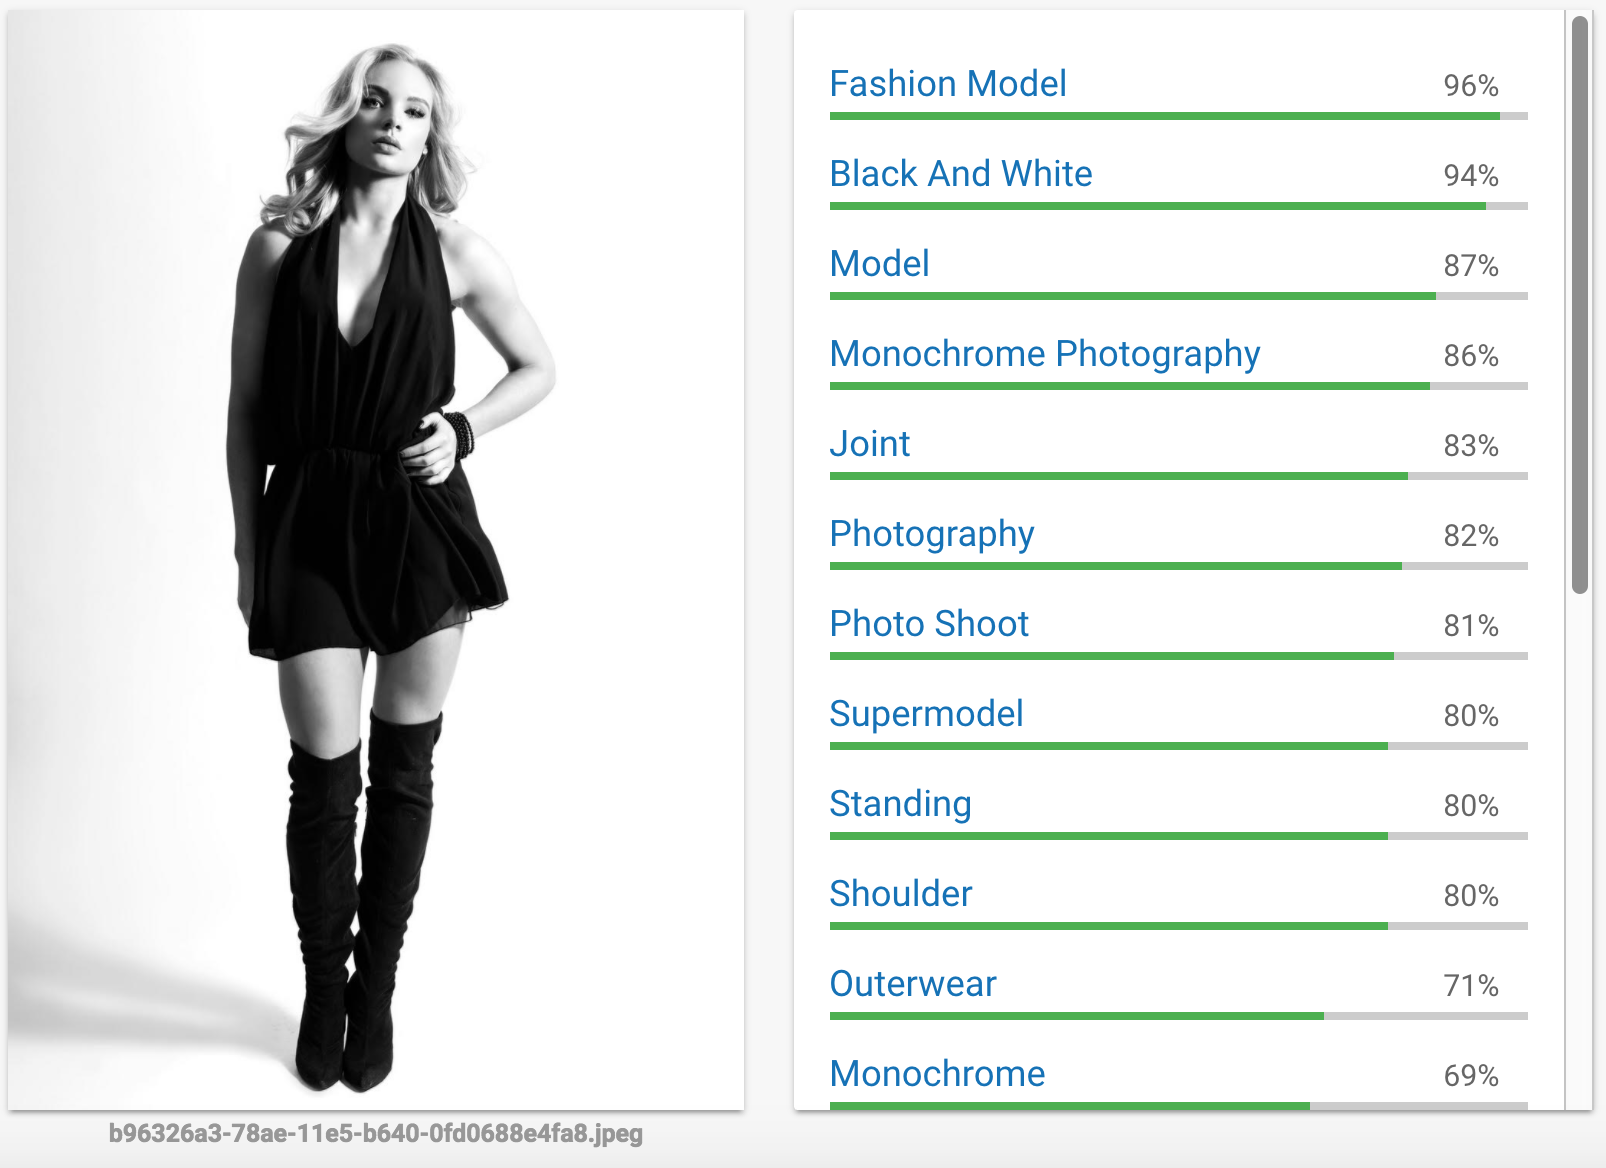
\includegraphics[width=0.6\textwidth]{images/google_vision_labels.png}
			\caption{The labels identified by the Google Vision API on one of the contest participant's image.}
			\label{google_vision_labels}
		\end{center}
	\end{figure}

\subsection{Methodology}
    % what kind of methods were chosen? 
    % what are the decisions behind the choices? 
    % what were the alternatives and why were they rejected? 

\subsection{Results}
    % what are the answers to RQ1? 
    % what are the answers to RQ2? 
    % what are the answers to RQ3?
    % what do the results mean? what are the implications? 